% !TeX spellcheck = en_US
%\documentclass[11pt,a4paper]{article}
\documentclass[11pt
  , a4paper
  , article
  , oneside
%  , twoside
%  , draft
]{memoir}

\usepackage{control}
\usepackage[numbers]{natbib}

\definecolor{babypink}{rgb}{0.96, 0.76, 0.76}
\definecolor{blizzardblue}{rgb}{0.67, 0.9, 0.93}

\begin{document}

\newcommand{\technumber}{
  RAON Control-Document Series\\
  Revision : v1.0,   Release : 2015-06-08 fixed date}
\title{\textbf{EPICS IOC를 위한 EPICS Records 사용법 및 그 개발 방법}}

\author{이상일\thanks{silee7103@ibs.re.kr},이정한\thanks{jhlee@ibs.re.kr}, 손창욱\thanks{cwson@ibs.re.kr},박미정\thanks{mijoy0909@ibs.re.kr}, 장효재\thanks{lkcom@ibs.re.kr}, 손형주\thanks{hjson@ibs.re.kr}, 남승희\thanks{namsh@ibs.re.kr} \\

  Rare Isotope Science Project\\
  Institute for Basic Science, Daejeon, South Korea
}
\date{\today}

\renewcommand{\maketitlehooka}{\begin{flushright}\textsf{\technumber}\end{flushright}}
%\renewcommand{\maketitlehookb}{\centering\textsf{\subtitle}}
%\renewcommand{\maketitlehookc}{C}
%\renewcommand{\maketitlehookd}{D}

\maketitle

\begin{abstract}
RAON accelerator는 대형 실험 장치로 많은 실험 장치들과 부대시설 장치로 구성되어 운영된다. 이러한 많은 실험 장치들을 제어하기 위한 제어 시스템들은 넓은 범위로 분산되어 구성되어 있으며 이러한 분산 환경에서의 많은 제어시스템들을 전체의 하나의 제어시스템으로 운영하기 위하여 RAON control system은 EPICS software framework을 사용한다. 본 문서는 EPICS 연계 시스템 인터페이스 개발자가 IOC를 개발하기 위하여 사용하는 EPICS record들에 대한 개발 가이드 레퍼런스를 제공하기 위함이다.
\end{abstract}

RAON accelerator에서 각 로컬 제어 시스템과 EPICS framework간의 integration을 위하여 가장 핵심이 되는 부분은 EPICS IOC 개발이다. 그만큼 EPICS의 여러 모듈 중에서 IOC는 그 핵심 모듈이라고 할 수 있다. IOC 모듈에서도 EPICS DB 생성을 위한 record의 사용 및 그 개발 방법은 제어 디바이스와 EPICS framework간의 인터페이스의 핵심이라 할 수 있다. 본 문서는 EPICS base에서 기본적으로 제공되는 records들에 대한 설명과 그 사용 예제를 통하여 IOC 설계 및 개발자들이 참고할 수 있는 가이드를 제시하려 함이며, 또한 base외에 추가적으로 개발된 IOC record의 개발 내용 및 사용 예제를 통하여 IOC record 개발을 체계성 및 일관성을 유지하여 향 후 체계적인 RAON control system software 형상관리에 도움을 주기위한 문서로 사용하기 위함이다.

\clearpage


\chapter{ai,ao}

\chapter{bi,bo}

\chapter{snmp}
SNMP(Simple Network Management protocol : 간이 망 관리 프로토콜)는 IP 네트워크상의 장치 및 장비들을 관리하고 모니티링하기 위한 인터넷 표준 프로코톨이다. 이는 네트워크 기반의 장비들의 효율적인 관리와 제어 시스템의 일관성, 최적화 기술의 습득 그리고 유지보수의 관점에서 도움이 될 것이다.
SNMP에 관한 간략한 정보는 아래와 같다.

\begin{itemize}
\item 인증과 암호화에 따른 차이를 가진 v1/2c/3의 세 가지 버전 지원
\item 관리되어야 할 장비에 대한 정보인 MIB (Management Information Base)가 필요
\item MIB 내 객체들은 고유 식별자 (Object Identfiers : OID)를 가짐 
\end{itemize}

SNMP는 MIB내 OID객체 데이터에 따라 INTEGER, unsigned INTEGER, TIMETICKS, IPADDRESS, OBJID, STRING, HEX STRING, DECIMAL STRING, BITS, unsigned int64, signed int64, float, double의 다양한 데이터 타입을 제공한다. 이는 기존의 EPICS가 제공하는 레코드 타입으로 표현할 수 있지만, 중이온가속기 제어 환경에 맞춘 독자적인 레코드 생성 및 이를 이용한 다양한 SNMP 데이터 처리를 위해 snmp, snmpstr Record가 개발되었다.

\section{레코드 구성 및 사용방법}
snmp, snmpstr support 모듈의 device type은 Listing \ref{list:lst1}과 같이 \textquotedblleft INST\_IO \textquotedblright 구조를 따른다.
\begin{lstlisting}[style=termstyle, escapechar=^, caption=snmpDevSoft.dbd파일, label={list:lst1}]]
include "snmpRecord.dbd"
include "snmpstrRecord.dbd"

device(snmp,INST_IO,devSNMPRead,"SNMP Read")
device(snmp,INST_IO,devSNMPWrite,"SNMP Write")
device(snmpstr,INST_IO,devSNMPRead_str,"SNMP Read")
\end{lstlisting}

또한, SNMP 사용을 위한 정보는 Listing \ref{list:lst2}와 같이 필드로 구성되어있다. 각 필드에 대한 자세한 설명은 다음 절을 참조바란다.
\begin{lstlisting}[style=termstyle, escapechar=^, caption=snmp·snmpstr 레코드의 일부, label={list:lst2}]]
typedef struct snmpRecord {
	char		host[81];	/* IP Address */
	char		comm[81];	/* Community */
	char		oids[81];	/* OID Name */
	char		auth[81];	/* auth password */
	char		priv[81];	/* priv password */
	char		vers[81];	/* SNMP Version */
	epicsFloat64	val;	/* Current Value */

{...}
} snmpRecord;

typedef struct snmpstrRecord {
	char		host[81];	/* IP Address */
	char		comm[81];	/* Community */
	char		oids[81];	/* OID Name */
	char		auth[81];	/* auth password */
	char		priv[81];	/* priv password */
	char		vers[81];	/* SNMP Version */
	char		val[40];	/* Current Value */
{...}
} snmpstrRecord;
\end{lstlisting}

\subsection{- snmpRecord}
이 레코드는 EPICS의 dbcommon.dbd에 정의된 기본 필드를 바탕으로 생성되어 레코드의 알람과 단위 등이 지원된다. 이는 SNMP의 String 타입을 제외한 모든 타입의 장비의 정보 값을 읽고, Integer 타입의 정보를 쓰는데 사용된다. snmpRecord는 SNMP 명령어 사용을 위해 기존의 필드 외 SNMP 명령어 사용에 필요한 필드를 추가한다. 이는 표 \ref{table:snmprecord}과 같으며 다음과 같은 목적을 가진다. HOST는 장비(Agent)의 주소로 IP 주소나 노드의 이름에 관한 필드이다. COMM은 v2c사용 시 Community String이며, v3 사용 시에 Username을 설정하는 필드이다. OID 필드는 읽거나 쓰고 싶은 장비의 정보 객체를 OID표기법이나 이름으로 설정한다. AUTH, PRIV는 v3 사용 시 암호화와 인증 비밀번호를 설정하는 필드이다. VERS는 레코드가 사용할 SNMP의 버전 설정 필드로 SNMPv2 사용 시 SNM과\_VERSION\_2c, v3 사용 시에는 SNMP\_VERSION\_3로 설정해야한다. OVAL은 레코드에 저장되어 있는 값으로 새로 쓰려는 값과 OVAL의 값이 같으면 설정은 변경되지 않는다. VAL는 최종적으로 PV가 가지는 장비의 정보 값이다.

\begin{table}[!h]
\begin{center}
\begin{tabular}{cccc}\hline
Field & Type & Description & Remark\\ \hline
HOST & String & Host Address \\ \hline
COMM & String & Community string (v2c) / Username (v3) \\ \hline
OIDS & String & OID Name \\ \hline
AUTH & String & Auth Key for strong authentication \\ \hline
PRIV & String & Priv Key for data encryption\\ \hline
VERS & String & SNMP Version & SNMPv2c/v3	 \\ \hline
OVAL & Double & Old Value \\ \hline
VAL & Double & Value \\ \hline
\end{tabular}
\caption{fields of snmpRecord}
\label{table:snmprecord} 
\end{center}
\end{table} 

APC사 Power Distribution Unit의 아웃렛 모니터링과 제어를 위한 snmp레코드 사용의 예는 다음과 같다.

{\scriptsize
\begin{verbatim}
record(snmp, "${A}:${P}_Outlet8_R") {
    field(DESC, "PDU outlet8 control")
    field(DTYP, "SNMP Read")
    field(SCAN, "5 second")
    field(VERS, "${V2C}")
    field(HOST, "${HOST}")
    field(COMM, "${COM}")
    field(OIDS, "${PO}sPDUOutletCtl.8")
}
record(snmp, "${A}:${P}_Outlet8_W") {
    field(DESC, "PDU outlet8 control")
    field(DTYP, "SNMP Write")
    field(SCAN, "5 second")
    field(VERS, "${V3}")
    field(AUTH, "${AUTH_P}")
    field(PRIV, "${PRIV_P}")
    field(HOST, "${HOST}")
    field(COMM, "${USER}")
    field(OIDS, "${PO}sPDUOutletCtl.8")
}
\end{verbatim}
}

\subsection{- snmpstrRecord}
snmpstrRecord는 Sting, BITS 타입의 데이터를 처리하기 때문에 알람 파라미터를 사용하지 않으며, 장비의 정보를 읽는 것만 가능하도록 생성되었다. 추후 Write를 지원할 예정이다. 필드에 대한 정보는 표 \ref{table:snmpstrrecord}와 같으며, OVAL, VAL 필드를 제외하고는 snmpRecord와 같다. 

\begin{table}[!h]
\begin{center}
\begin{tabular}{cccc}\hline
Field & Type & Description & Remark\\ \hline
HOST & String & Host Address \\ \hline
COMM & String & Community string (v2c) / Username (v3) \\ \hline
OIDS & String & OID Name \\ \hline
AUTH & String & Auth Key for strong authentication \\ \hline
PRIV & String & Priv Key for data encryption\\ \hline
VERS & String & SNMP Version & SNMPv2c	 \\ \hline
VAL & String & Value \\ \hline
\end{tabular}
\caption{fields of snmpstrRecord}
\label{table:snmpstrrecord} 
\end{center}
\end{table} 

아래는 APC PDU Outlet의 이름을 모니터링하는 snmpstr레코드의 사용 예이다. 

{\scriptsize
\begin{verbatim}
record(snmpstr, "${A}:${P}_Outlet8_Name") {
    field(DESC, "PDU outlet8 Name")
    field(DTYP, "SNMP Read")
    field(SCAN, "5 second")
    field(VERS, "${V2C}")
    field(HOST, "${HOST}")
    field(COMM, "${COM}")
    field(OIDS, "${PO}sPDUOutletCtlName.8")
}
\end{verbatim}
}


\chapter{motor}

\chapter{asyn}

\chapter{rdbpostgreSQL}

rdbpostgreSQL record의 개발 목적은 아래와 같다.
\begin{itemize}
	\item EPICS IOC의 값을 DBMS에서 제공하는 풍부한 연산 알고리즘 활용하여 계산
	\item EPICS로 구성된 가속기 operation parameters 들을 자동으로 Database화 하여 관리
	\item 향 후 가속기 Alarm 시스템과 통신사의 SMS DB와 연계하여 해당 운전자 그룹에 자동 Alarm Message 전송
\end{itemize}

\chapter{rdbmySQL}
SRF Test Facility에서 RMS(Radiation Monitoring System)는 radiation 관련 모니터링 데이터를 MySQL 데이터베이스에 저장한다. 이 저장된 radiation 정보를 통합 operation 관점에서 상시 모니터링 되어야 하므로 MySQL의 데이터베이스와 EPICS간의 인터페이스를 위한 record이다.

rdbmySQL record의 개발 목적은 아래와 같다.
\begin{itemize}
	\item MySQL 데이터베이스와의 interface.
	\item EPICS로 구성된 가속기 operation parameters 들을 자동으로 Database화 하여 관리
\end{itemize}

그림 \ref{fig:rms_epics_db}는 rdbmySQL record를 이용하여 RMS t\_values 테이블과 인터페이스하기 위하여 EPICS db를 구성하는 예를 보여준다. 현 문지동 SRF Test Facility에는 Radiation Monitoring을 위한 시스템이 구축 되어 운영 중이다. 이 시스템은 방사능 모니터링 디바이스로 부터 나오는 측정 값을 RS 485 시리얼 통신을 통해 획득하며 그 데이터를 MySQL 데이터 베이스에 저장한다. 이는 해당 데이터를 계속적으로 MySQL 테이블에 insert 하는 형태이며, EPICS PV화를 위해서는 항상 마지막 insert 데이터를 쿼리해야 하는 상황이다. 해당 부분을 좀 더 효과적으로 하기 위한 방안으로 해당 테이블의 insert transaction이 발생할 경우 MySQL trigger를 발생시켜 해당 테이블에 특정 필드 값만을 새롭게 테이블로 구성하여 insert transaction의 값을 새로운 테이블에 update 시킨다. 이 경우 EPICS PV interface를 위한 rdbmySQL record는 항상 새롭게 update되는 테이블에 쿼리하여 향 후 수만 개 이상의 데이터가 쌓이더라도 RMS 실시간 데이터를 보기위한 비용은 거의 없이 EPICS로 처리 할 수 있다. 해당 record를 "I/O Intr"로 설정시 insert transaction 처리 전에 update를 거치며 거의 최대 0.1 sec 이내 EPICS PV와 동기화 되어 작동된다.

RMS 방사능 측정 데이터 테이블 t\_values에 대한 insert transaction에 대한 MySQL trigger 발생은 아래와 같이 구성 할 수 있다.


\begin{lstlisting}[style=termstyle]
mysql> create table t_values_epics (E_ID int, InDate datetime, ChannelNo int, Value1 varchar(20), Value2 varchar(20));
Query OK, 0 rows affected (0.14 sec)

mysql> insert into t_values_epics(E_ID,InDate,ChannelNo,Value1,Value2) values(3,curdate(),2,1.2323, 3.4563);
Query OK, 1 row affected (0.04 sec)

mysql> select * from t_values_epics;
+------+---------------------+-----------+--------+--------+
| E_ID | InDate              | ChannelNo | Value1 | Value2 |
+------+---------------------+-----------+--------+--------+
|    3 | 2015-06-05 00:00:00 |         2 | 1.2323 | 3.4563 |
+------+---------------------+-----------+--------+--------+
1 row in set (0.00 sec)

mysql> delimiter //
mysql> create trigger rms_epics_tri before insert on t_values for each row begin update t_values_epics set E_ID=new.E_ID, InDate=new.InDate, ChannelNo=new.ChannelNo, Value1=new.Value1, Value2=new.Value2; end //
Query OK, 0 rows affected (0.10 sec)

mysql> delimiter ;

mysql> select * from t_values_epics;
+------+---------------------+-----------+--------+--------+
| E_ID | InDate              | ChannelNo | Value1 | Value2 |
+------+---------------------+-----------+--------+--------+
|    3 | 2015-06-05 00:00:00 |         2 | 1.2323 | 3.4563 |
+------+---------------------+-----------+--------+--------+
1 row in set (0.00 sec)

mysql> INSERT INTO `t_values` VALUES (1,'2015-06-03 12:20:17',1,'0.165296E+0','','1','20150603','122017','0','0',1,'',NULL);
ERROR 1062 (23000): Duplicate entry '1-2015-06-03 12:20:17-20150603-122017' for key 'PRIMARY'

mysql> INSERT INTO `t_values` VALUES (3,'2015-06-07 12:20:19',2,'3.1534','45.2323','4','20150607','122019','0','0',1,'',NULL);
Query OK, 1 row affected (0.06 sec)

mysql> select * from t_values_epics;
+------+---------------------+-----------+--------+---------+
| E_ID | InDate              | ChannelNo | Value1 | Value2  |
+------+---------------------+-----------+--------+---------+
|    3 | 2015-06-07 12:20:19 |         2 | 3.1534 | 45.2323 |
+------+---------------------+-----------+--------+---------+
1 row in set (0.00 sec)

$>camonitor  MYSQL_RMS_EID MYSQL_RMS_INDATE MYSQL_RMS_CHANNELNO MYSQL_RMS_VALUES1 MYSQL_RMS_VALUES2

MYSQL_RMS_EID                  2015-06-05 13:57:26.969823 1  
MYSQL_RMS_INDATE               2015-06-05 13:57:26.969839 2015-06-05 12:20:17  
MYSQL_RMS_CHANNELNO            2015-06-05 13:57:26.969844 1  
MYSQL_RMS_VALUES1              2015-06-05 13:57:26.969846 0.165296E+0  
MYSQL_RMS_VALUES2              2015-06-05 13:57:26.969848   
MYSQL_RMS_INDATE               2015-06-05 13:57:54.095276 2015-06-05 12:20:18  
MYSQL_RMS_VALUES2              2015-06-05 13:57:54.095281 0.3534  
MYSQL_RMS_EID                  2015-06-05 13:58:58.558086 2  
MYSQL_RMS_INDATE               2015-06-05 13:58:58.558092 2015-06-05 12:20:19  
MYSQL_RMS_CHANNELNO            2015-06-05 13:58:58.558093 2  
MYSQL_RMS_VALUES1              2015-06-05 13:58:58.558094 0.1534  
MYSQL_RMS_VALUES2              2015-06-05 13:58:58.558095 5.2323  
MYSQL_RMS_EID                  2015-06-08 08:25:23.384936 3  
MYSQL_RMS_INDATE               2015-06-08 08:25:23.384960 2015-06-07 12:20:19  
MYSQL_RMS_VALUES1              2015-06-08 08:25:23.384969 3.1534  
MYSQL_RMS_VALUES2              2015-06-08 08:25:23.384973 45.2323  
\end{lstlisting}

DB 구성 및 사용방법:

rdbmySQL record는 INP, INPA to INPL까지 총 13개의 입력 필드를 갖는다. 해당 입력필드는 QRY 필드에 작성되는 query문의 필드 순서에 따른 SQL query가 작성 된다. 쿼리 실행에 대한 데이터 타입은 인터페이스 되는 MySQL 테이블의 필드에 대한 데이터 타입을 확인하여 INP 링크에 연결되는 EPICS record의 데이터 타입를 설정한다. 그림 \ref{fig:rms_epics_db}에 대한 예를 설명하면 아래와 같다.

\begin{lstlisting}[style=termstyle]
record(stringin, "$(SYS)_RMS_INDATE") {
	field(SCAN, "Passive")
}
record(longin, "$(SYS)_RMS_EID") {
	field(SCAN, "Passive")
}
record(longin, "$(SYS)_RMS_CHANNELNO") {
	field(SCAN, "Passive")
}
record(stringin, "$(SYS)_RMS_VALUES1") {
	field(SCAN, "Passive")
}
record(stringin, "$(SYS)_RMS_VALUES2") {
	field(SCAN, "Passive")
}
record(rdbmySQL, "$(SYS):READ_RMS") {
	field(SCAN, "I/O Intr")
	field(PINI, "YES")
	field(DTYP, "ReadData")
	field(QRY, "select E_ID, InDate, ChannelNo, Value1, Value2 from t_values_epics")
	field(INP, "$(SYS)_RMS_EID")
	field(INPA, "$(SYS)_RMS_INDATE")
	field(INPB, "$(SYS)_RMS_CHANNELNO")
	field(INPC, "$(SYS)_RMS_VALUES1")
	field(INPD, "$(SYS)_RMS_VALUES2")
}
\end{lstlisting}
상위의 rdbmySQL record "\$(SYS):READ\_RMS"에서 QRY 필드는 200자 까지의 SQL query문을 작성할 수 있다.  QRY에 작성된 "select E\_ID,InDate,ChannelNo,Value1,Value2 from t\_values\_epics" 는  t\_values\_epics 테이블로 부터 각 필드가 순서대로 INP, INPA, INPB, INPC, INPD의 Input link PV와 연결된다. 따라서 각 필드의 데이터 타입에 따라 INP 링크에 연결된 PV의 record 타입을 설정한다. 아래는 t\_values\_epics 테이블에 대한 각 필드의 데이터 타입을 보여준다.

\begin{lstlisting}[style=termstyle]
mysql> desc t_values_epics;
+-----------+-------------+------+-----+---------+-------+
| Field     | Type        | Null | Key | Default | Extra |
+-----------+-------------+------+-----+---------+-------+
| E_ID      | int(11)     | YES  |     | NULL    |       |
| InDate    | datetime    | YES  |     | NULL    |       |
| ChannelNo | int(11)     | YES  |     | NULL    |       |
| Value1    | varchar(20) | YES  |     | NULL    |       |
| Value2    | varchar(20) | YES  |     | NULL    |       |
+-----------+-------------+------+-----+---------+-------+
\end{lstlisting}

여기서 INP와 link된 EPICS PV record 타입은 longin이며, INPA는 string 형태의 날짜를 보여주기 위하여 stringin, INPB는 longin, INPC와 INPD는 ai record가 사용되었다. 해당 INP 링크는 DB scan이 processing passive로 설정되어 rdbmySQL scan rate을 따른다. rdbmySQL record "\$(SYS):READ\_RMS"가 "I/O Intr"로 설정되면, MySQL insert transaction과 최대 0.1sec로 scan offset을 발생한다. 또한, rdbmySQL record의 값은 0, -1값을 가질 수 있으며 0의 경우는 SQL query 수행이 정상적으로 fetch 되었음을 의미하며, -1의 값을 SQL query 실행에 문제가 있어 정상적인 값을 fetch 하지 못했음을 의미한다.

st.cmd 실행 방법:
아래와 같이 st.cmd 스크립트 내에 MySQL database와 connection을 위한 drvMySQLConnInit을 아래 파라미터 정보에 맞게 추가한다.

\begin{lstlisting}[style=termstyle]
#!../../bin/linux-x86_64/rdbmysql

## You may have to change rdbmysql to something else
## everywhere it appears in this file

< envPaths

cd "${TOP}"

## Register all support components
dbLoadDatabase "dbd/rdbmysql.dbd"
rdbmysql_registerRecordDeviceDriver pdbbase

# parameters: dbname, username, password, host to connect, port to connect
#drvMySQLConnInit("dbname","username","password","hostip","port");
#drvMySQLConnInit("epics_db","root","qwer1234","127.0.0.1","3306");
drvMySQLConnInit("rad_inst","root","qwer1234","127.0.0.1","3306");

#dbLoadRecords("db/MYSQL_EPICS.vdb","SYS=MYSQL")
dbLoadRecords("db/RMS_EPICS.vdb","SYS=MYSQL")

cd "${TOP}/iocBoot/${IOC}"
iocInit
\end{lstlisting}

아래 그림 \ref{fig:rms_epics_view_trigger}은 MySQL t\_values 테이블의 insert transaction 시 t\_values\_epics 테이블이 triggering update 됨을 보여준다.

\clearpage

\begin{figure}[h!]
	\centering
	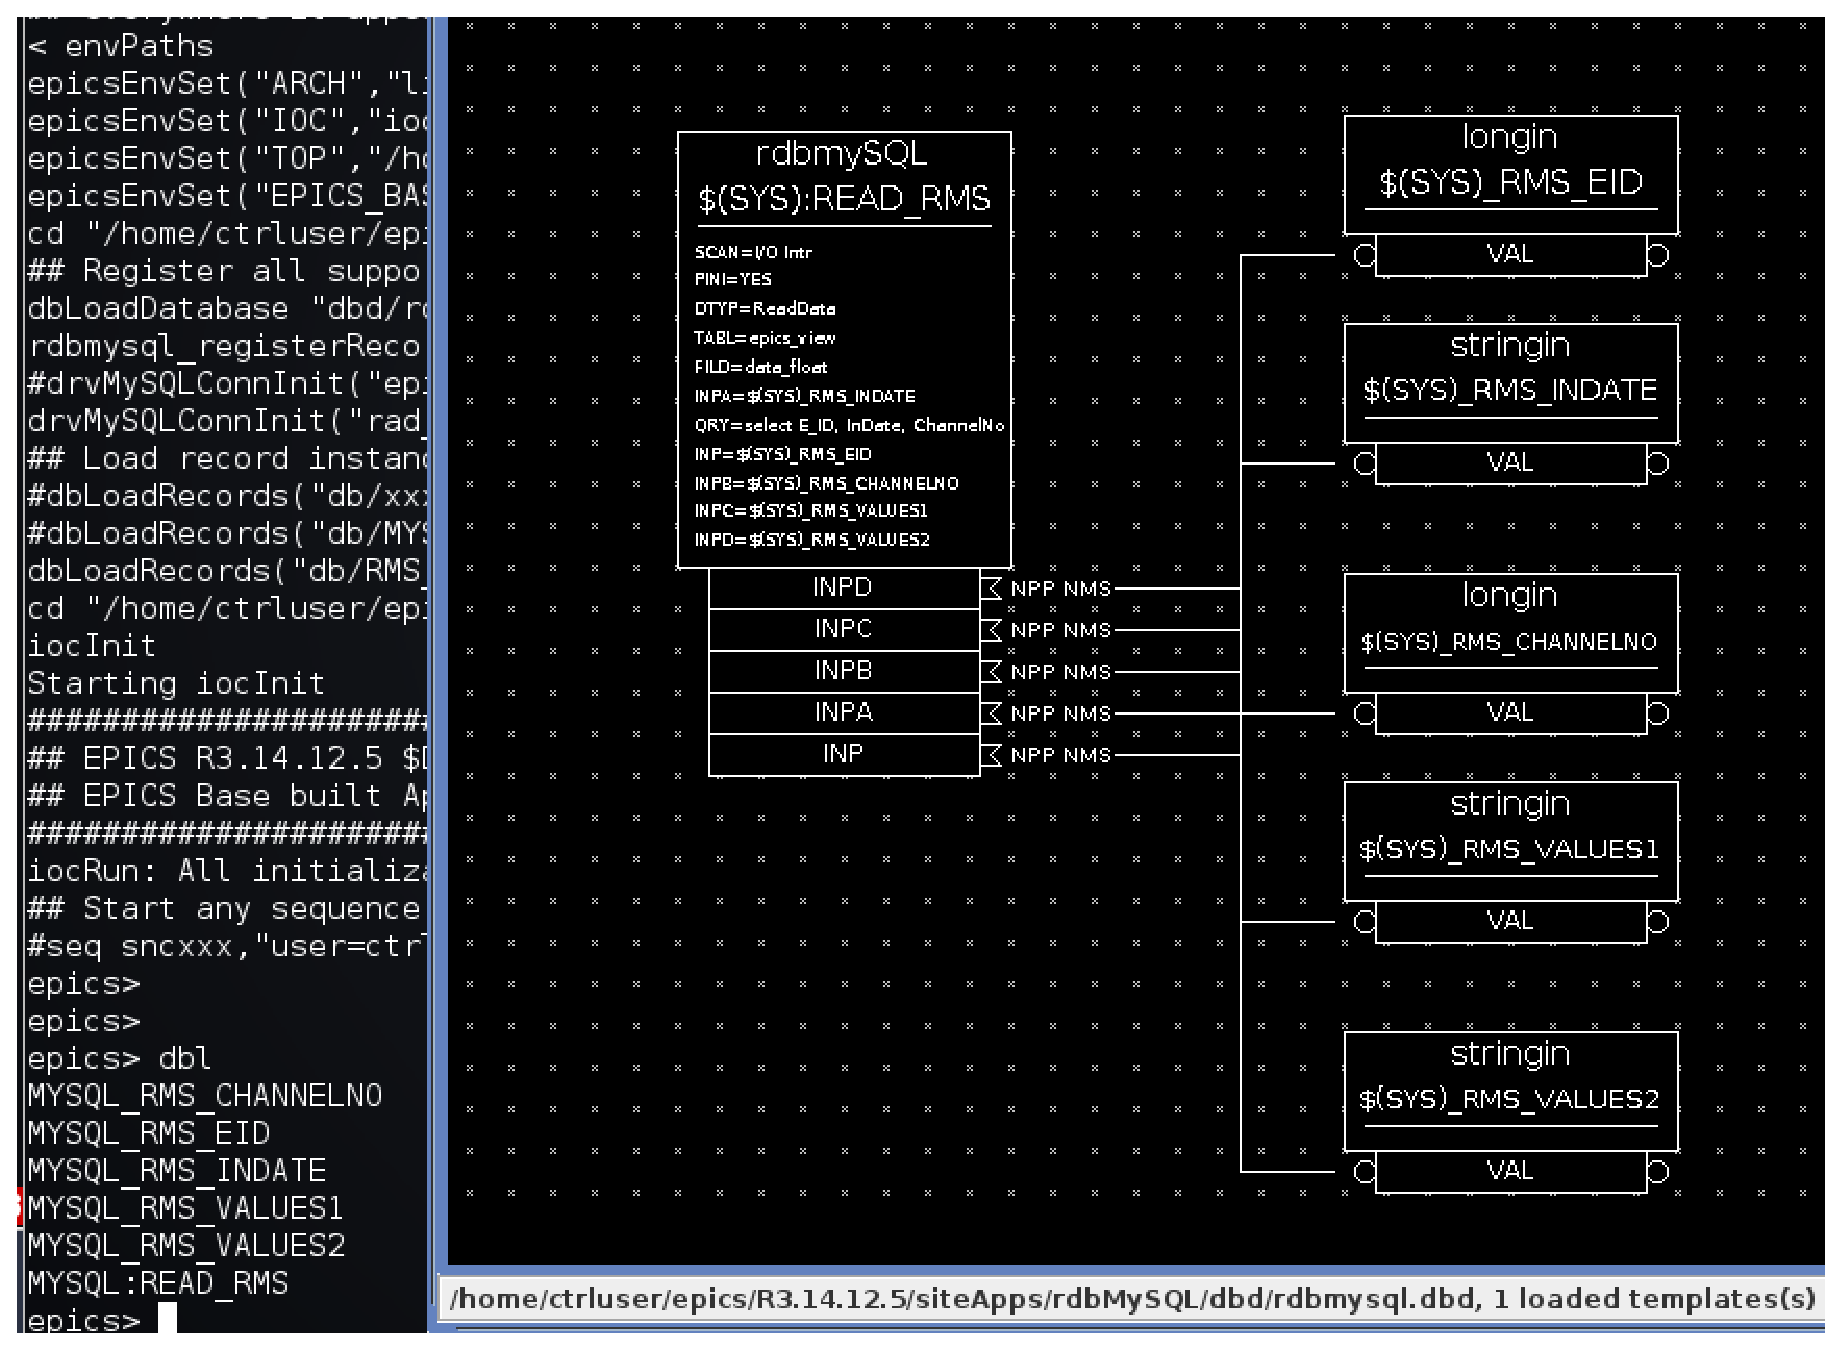
\includegraphics[width=0.7\textwidth]{./images/rms_epics_db.eps}
	\caption{RMS MySQL 인터페이스를 위한 EPICS DB설정}
	\label{fig:rms_epics_db}
\end{figure}

\begin{figure}[h!]
	\centering
	\includegraphics[width=0.7\textwidth]{./images/rms_epics_view_trigger.eps}
	\caption{MySQL 트리거링을 이용한 RMS View Table}
	\label{fig:rms_epics_view_trigger}
\end{figure}

\clearpage

\chapter{ifstat}
EPICS IOC는 ethernet based의 분산 제어 software framework로 불린다. 이는 ethenet으로 연결된 IOC는 항상 데이터 패킷을 발생 시키는데 해당 데이터 패킷이 얼마나 발생하는지 로컬 ethernet에 대한 패킷량을 계산하여 PV화 한다. 이는 네트워크 모니터링 용으로 사용 될 수 있으며, 향 후 IOC의 네트워크에 대한 건전성을 모니터링하는데 적용 할 수 있다.


\chapter{Hardware에 따른 EPICS device/driver}
\section{RTP}
RTP hardware에 대한 IOC 구성은 해당 IOC 개발 문서를 참조하며, 본 절에서는 DB를 구성하는 방법을 간략하게 설명한다.

아래 그림 \ref{fig:rtp_db}에서 처럼 RTP HW와 EPICS device support 모듈과 인터페이스 하기 위한 DB 작성을 보여준다. RTP HW는 상위 어플리케이션을 위하여 ethernet 기반의 통신(UDP,TCP)을 사용한다. 해당 RTP HW 카드에 따른 tcp socket 통신 프로토콜은 open되어 사용되며, IOC 개발 문서에 설명되었다. 해당 RTP device support 모듈은 크게 ai/ao, longin/longout, bi/bo 3가지 형태의 데이터 타입을 가질 수 있으며, 인터페이스를 위한 DB 작성을 아래와 같다.

\begin{lstlisting}[style=termstyle]
record(ai, RTP_AI_TEST) {
field(SCAN, "1 second")
field(PINI, "YES")
field(DTYP, "rtpSyncReadAI")
field(VAL, "0")
field(INP, "@RTP(0,95)")
}
record(bi, RTP_BI_TEST) {
field(DESC, "Bool value")
field(SCAN, "1 second")
field(PINI, "YES")
field(DTYP, "rtpSyncReadBI")
field(INP, "@RTP(0,485)")
field(ZNAM, "OFF")
field(ONAM, "ON")
}
record(ao, RTP_AO_TEST) {
field(DESC, "AO Test")
field(DTYP, "rtpSyncReadAO")
field(OUT, "@RTP(0,97)")
}
record(bo, RTP_BO_TEST) {
field(DESC, "RTP BO Test")
field(DTYP, "rtpSyncReadBO")
field(OUT, "@RTP(0,517)")
field(ZNAM, "OFF")
field(ONAM, "ON")
}
\end{lstlisting}

상위에서 처럼 INP 또는 OUT에서 작성되는 방법은 "@RTP(cpu\_number, index\_number)" 이다. cpu node number는 RTP cpu node 설정 방법에 따라 redundant 구성 등에 의해 변경 될 수 있지만 일반적으로는 "0"을 갖는다. 또한 index number 역시 RTP 구성 등에 의해 Hardware index와 동일 하여야 한다. RTP Hardware Tag index와 관련하여는 RTP 문서를 참조한다. 해당 Hardware index는 RTP에서 제공한 NetArrays 소프트웨어 툴에서 확인 가능하다. 위에서 나오는 index number는 NetArrays를 통해 확인한 index number이며 구성에 따라 변경 될 수 있다.

\begin{figure}[h!]
	\centering
	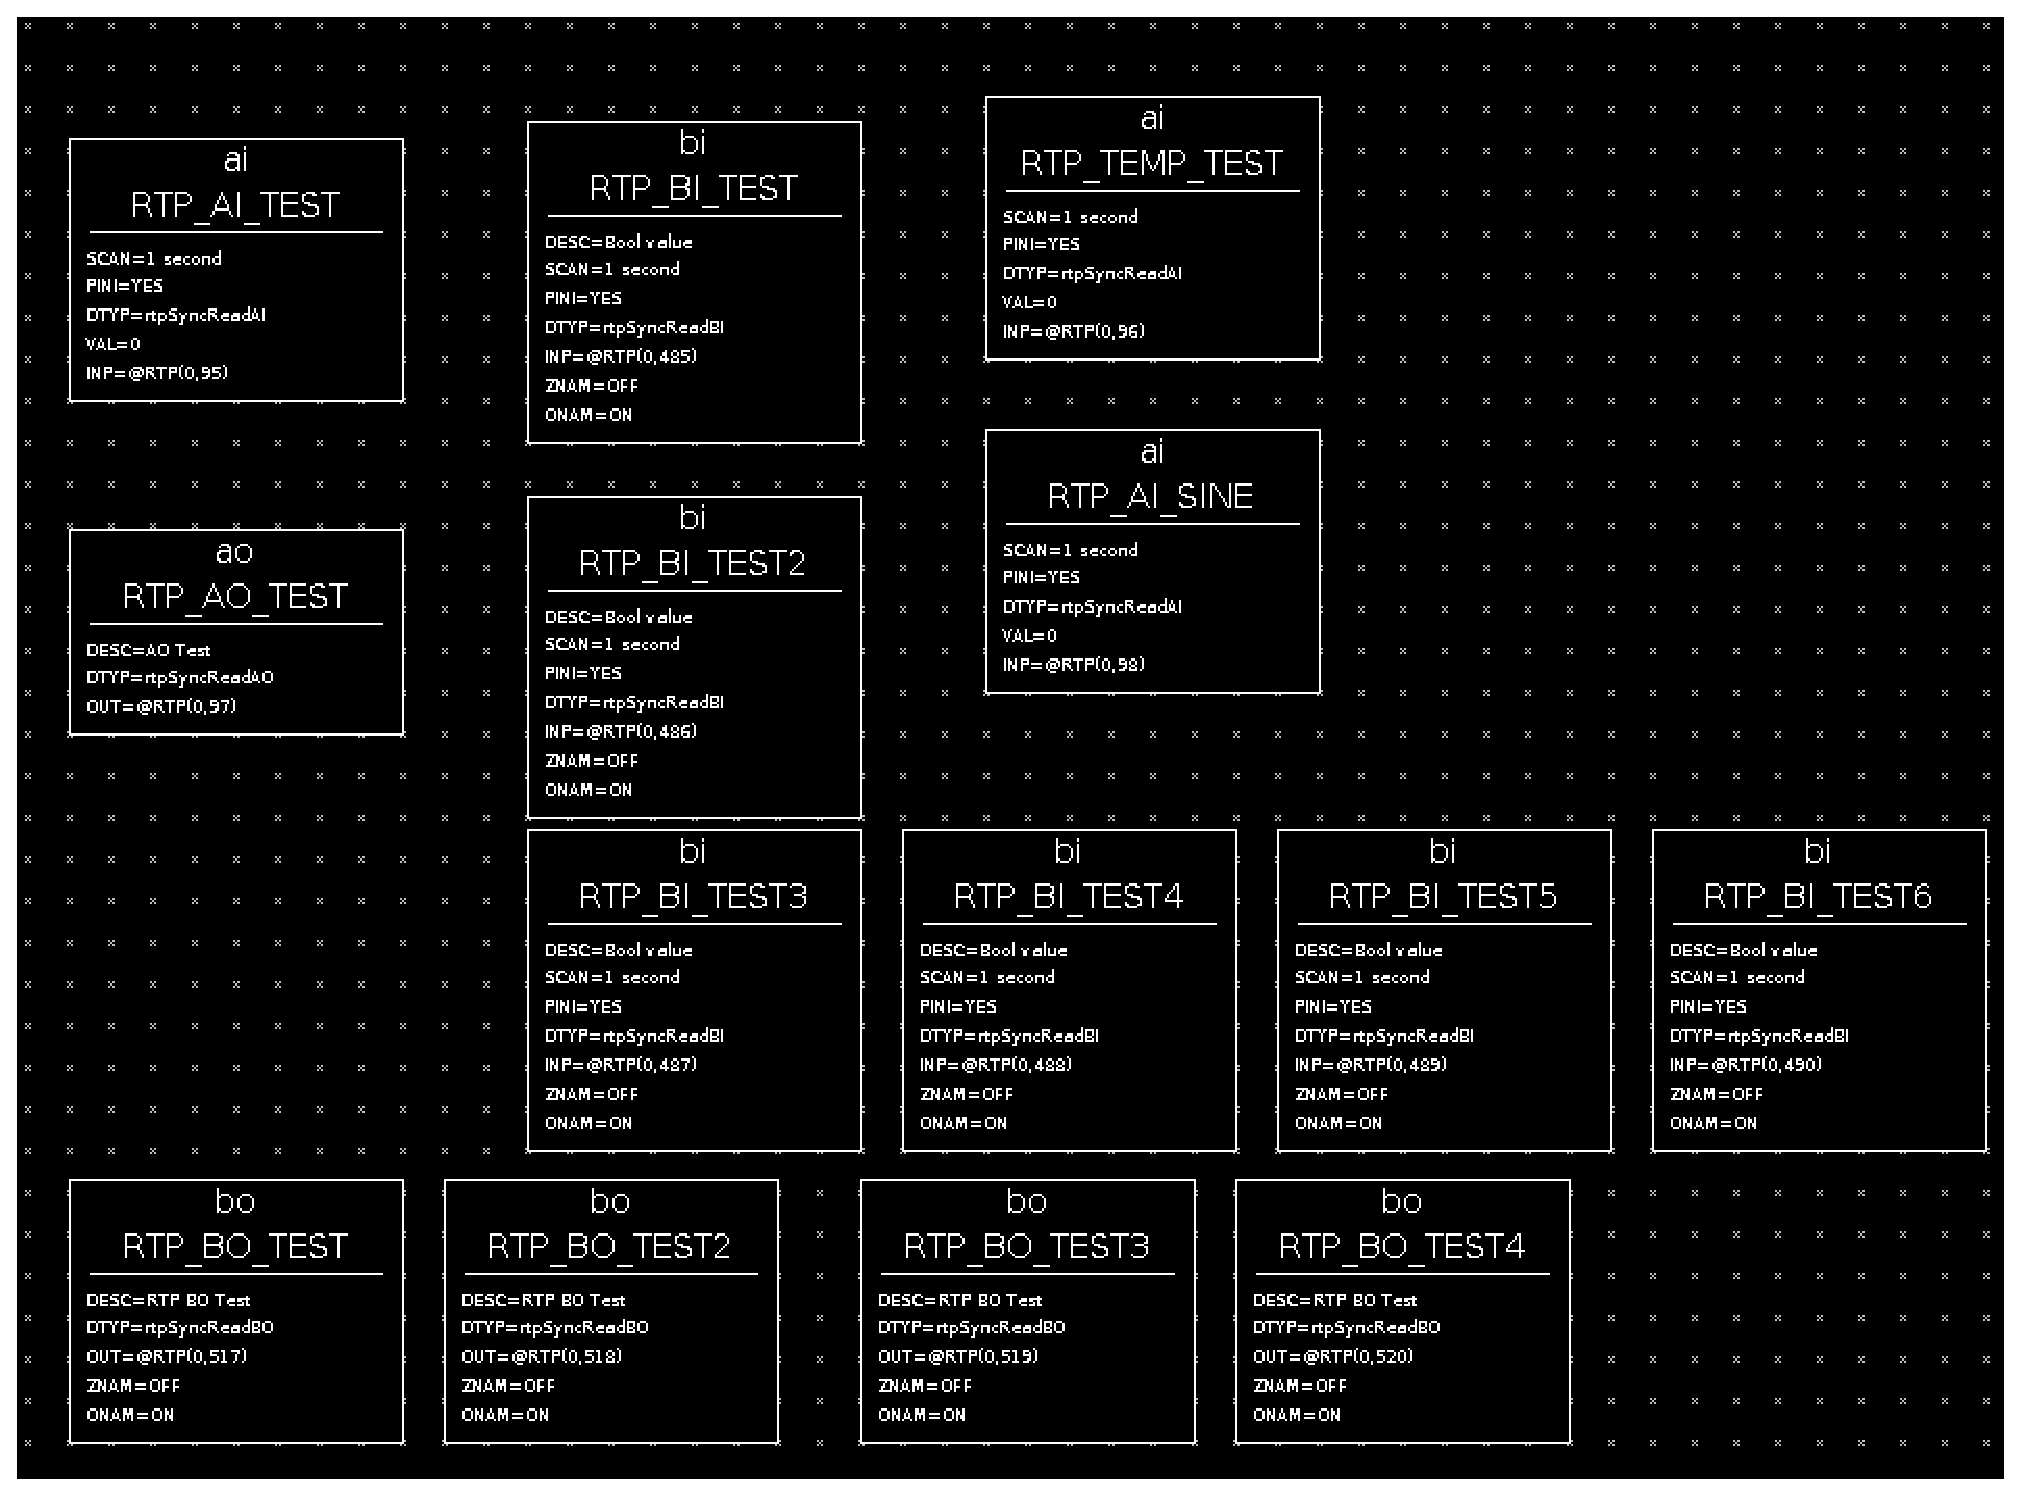
\includegraphics[width=0.85\textwidth]{./images/rtp_db.eps}
	\caption{RTP interface database}
	\label{fig:rtp_db}
\end{figure}

RTP device support 모듈의 device type은 아래와 같이 "INST\_IO" 구조를 따른다.
\begin{lstlisting}[style=termstyle]
device(ai,INST_IO,devSyncRTPReadAI,  "rtpSyncReadAI")
device(ao,INST_IO,devSyncRTPReadAO,  "rtpSyncReadAO")
device(bi,INST_IO,devSyncRTPReadBI,  "rtpSyncReadBI")
device(bo,INST_IO,devSyncRTPReadBO,  "rtpSyncReadBO")
device(longin,INST_IO,devSyncRTPReadLI,  "rtpSyncReadLI")
\end{lstlisting}


st.cmd 실행 방법:
아래와 같이 st.cmd 스크립트 내에 RTP Node Processor와의 connection을 위한 drvSyncRTPConfigure를 아래 파라미터 정보에 맞게 추가한다.

\begin{lstlisting}[style=termstyle]
#!../../bin/linux-x86_64/rtp

< envPaths

cd ${TOP}

## Register all support components
dbLoadDatabase "dbd/rtp.dbd"
rtp_registerRecordDeviceDriver pdbbase

#drvAsynIPPortConfigure("portName","hostInfo(e.g. IP:port protocol", priority, noAutoConnect)
drvSyncRTPConfigure("RTPDevice", "89.89.80.30:50199 TCP", 0, 0)

## Load record instances
#dbLoadRecords("db/xxx.db","user=sileeHost")
dbLoadRecords("db/RTPTest.vdb")
#dbLoadRecords("db/RTPOneTest.vdb")

cd ${TOP}/iocBoot/${IOC}
iocInit
\end{lstlisting}

\clearpage
\bibliographystyle{unsrtnat}
\bibliography{./refs}

\end{document}

